\documentclass[a4paper,12pt]{article}
\usepackage[T2A]{fontenc}
\usepackage[utf8]{inputenc}
\usepackage[english, russian]{babel}
\usepackage{minted}
\usepackage{verbatim}
\usepackage{graphicx}
\usepackage{caption}
\usepackage{subcaption}
\usepackage[left=2.5cm,right=2.5cm,top=2cm,bottom=2cm]{geometry}

\newenvironment{longlisting}{\captionsetup{type=listing}}{}

\newenvironment{pseudolisting}
 {\begin{minipage}{\linewidth}\vspace*{\topsep}}
 {\vspace*{\topsep}\end{minipage}}

\begin{document}

\begin{titlepage}
  \begin{center}
    \large
     
    \textbf{}

 

    
    \vfill
     
     
   
    \vfill
 
    \textsc{Лаборатная работа, вариант №24}\\[5mm]
     
    {\LARGE Теория погрешностей и машинная арифметика\\[2mm]
    }
    \textsc{Задания: 1.1.24, 1.5.6, 1.6, 1.7, 1.9.6}\\[5mm]
  \bigskip
     
    
\end{center}
\vfill
 

 
\hfill\begin{flushright}
  \textbf{Студент:}\\
  Паршина Софья Романовна \\
  3 курс, группа БПМ213
\end{flushright}%
\vfill

\end{titlepage}


\tableofcontents

\section{Частичные суммы ряда(1.1.24)}
\subsection{Формулировка задачи}
Дан ряд  $$\sum_{n=0}^\infty a_n,$$ надо найти сумму аналитически как предел частичных сумм S(N), затем вычислить частичные суммы в зависимости от N={10, ..., $10^5$} и сравнить абсолютную погрешность и кол-во верных цифр в частичной сумме.
   $$S(N) = \sum_{n=0}^N a_n$$
   $$a_n = \frac{96}{n^2 +9n + 20}$$
   
\subsection{Аналитический расчет суммы ряда}
Выпишем формулу суммы ряда:
   $$S = \sum_{n=0}^{\infty} \frac{96}{n^2 +9n + 20}$$ 
 
   $$S_N = \sum_{n=0}^{N} \frac{96}{n^2 +9n + 20} = \sum_{n=0}^{N} \frac{96}{(n+4)(n+5)} = 96 * \sum_{n=0}^{N} (\frac{1}{n+4}-\frac{1}{n+5}) = 96 * (\frac{1}{4}-\frac{1}{N+5}),$$
   $$S = \lim_{n\rightarrow \infty}S_N = 24 - 0 = 24$$
Ответ: $$S = \sum_{n=0}^{\infty} \frac{96}{n^2 +9n + 20} = 24$$

\subsection{Код на Python}

\begin{longlisting}
\inputminted{python}{partial_sums_of_a_series.py}
\end{longlisting}

\subsection{Результат работы программы}
\begin{longlisting}
\verbatiminput{series_result.txt}
\end{longlisting}

\subsection{Графики точности результата}
\begin{figure}[H]
\centering
\begin{subfigure}{.5\textwidth}
  \centering
  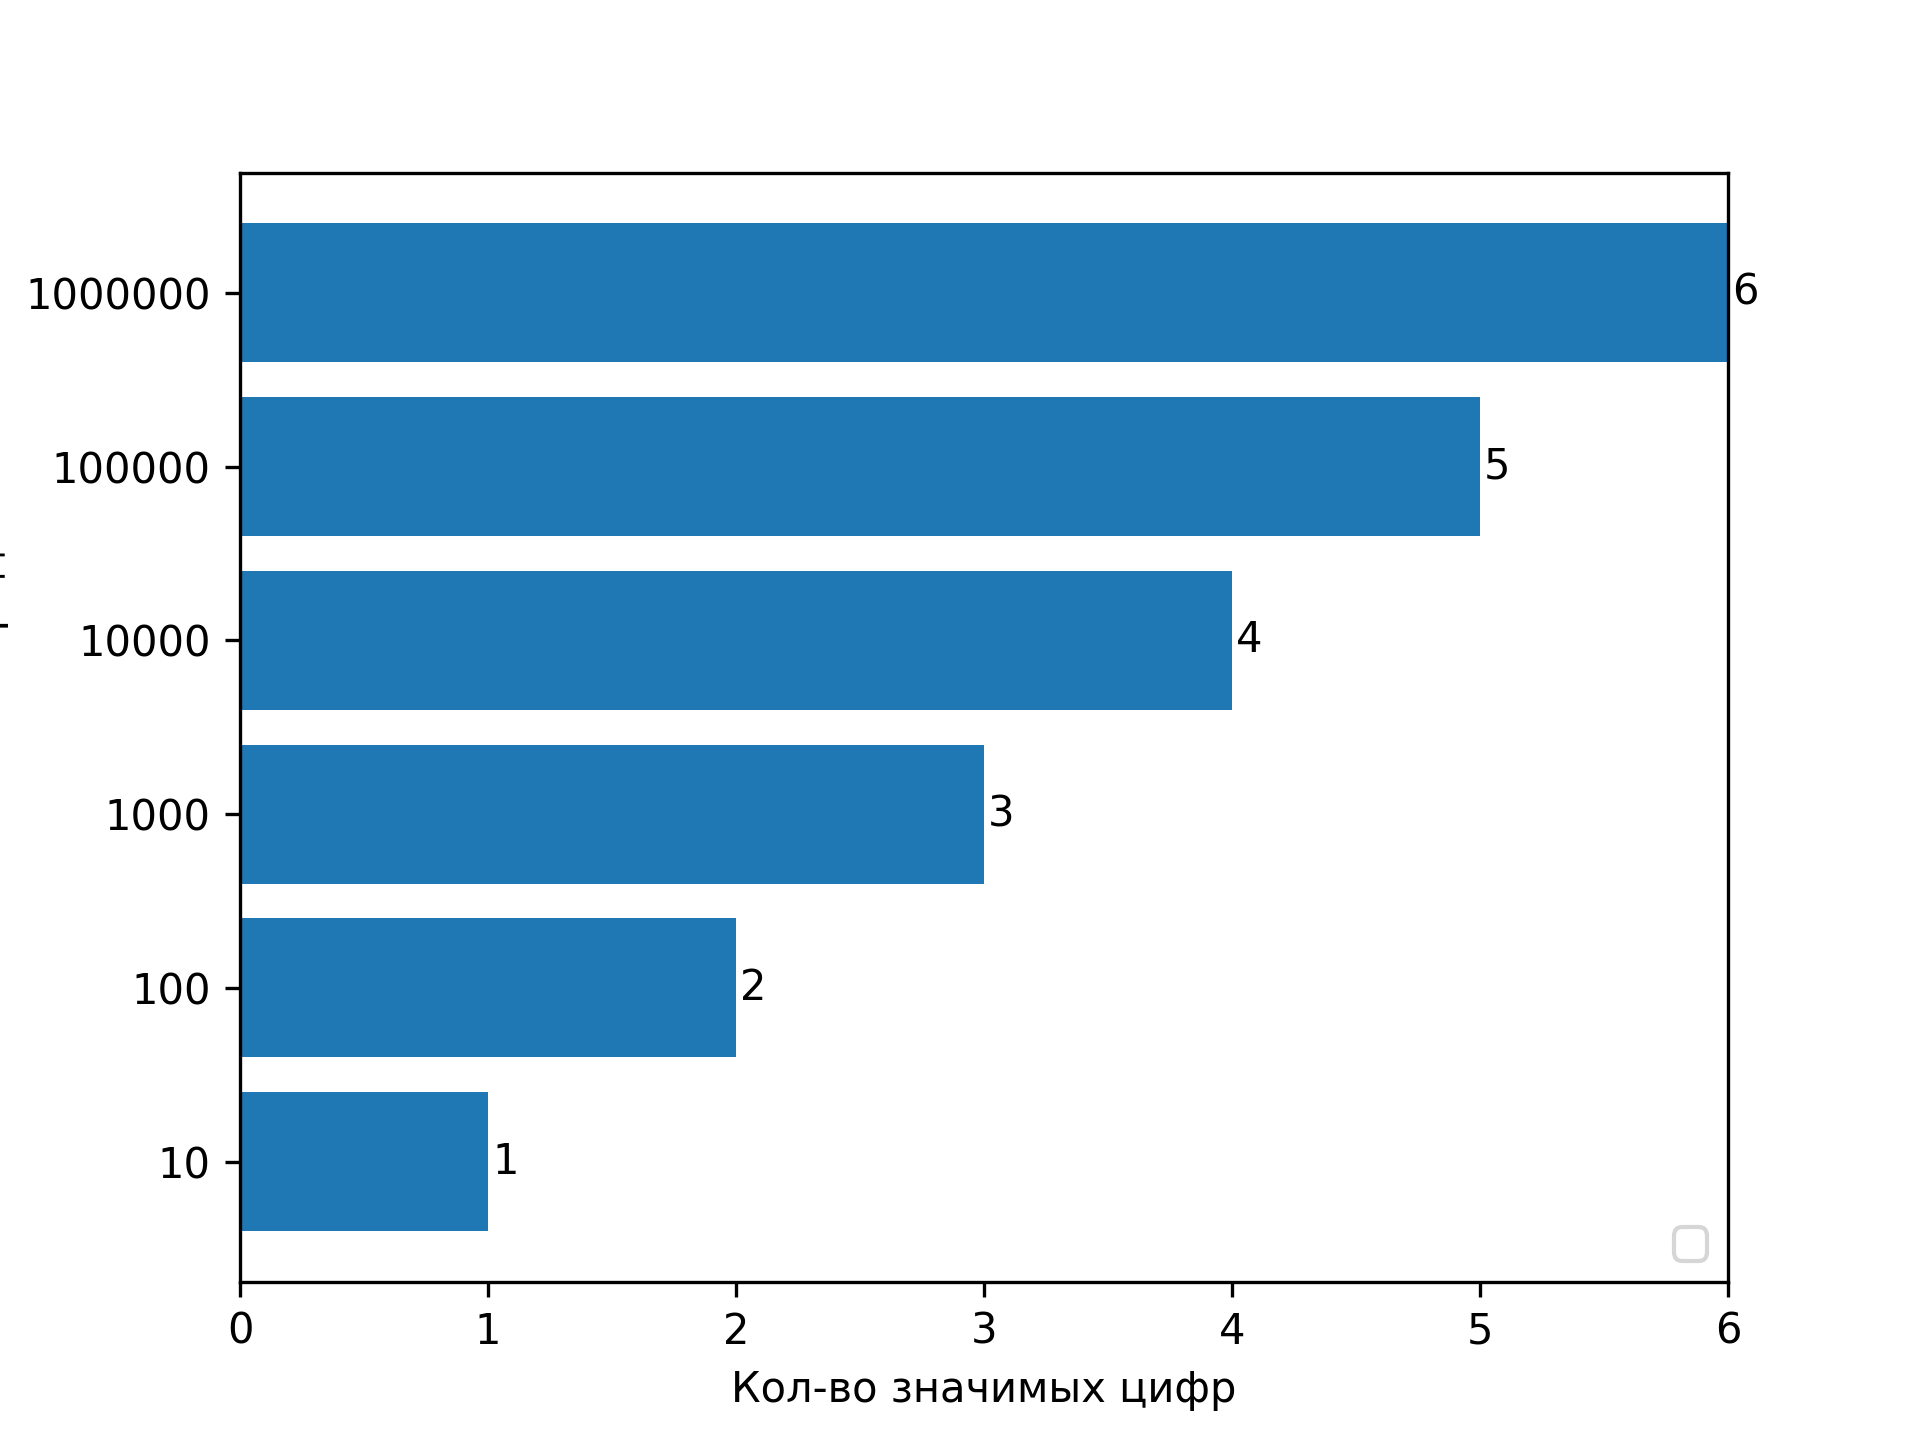
\includegraphics[width=\linewidth]{right_figure_partial sums of a series(plot).png}
  \label{fig:sub1}
\end{subfigure}%
\caption{Точность в зависимости от N}
\label{fig:test}
\end{figure}

\section{Квадратное уравнение(1.5.6)}
\subsection{Формулировка задачи}
Дано квадратное уравнение. Предполагается, что один из коэффициентов уравнения (помечен $*$) получен в результате округления. Произвести теоретическую оценку погрешностей корней в зависимости от погрешности коэффициента. Вычислить корни уравнения при нескольких различных значениях коэффициента в пределах заданной точности, сравнить.
$$x^2+bx+c = 0$$
$$b = -3.29$$
$$c^* = 2.706 $$
    
\subsection{Теоретическая оценка погрешности}

Выпишем формулу уравнения и погрешности переменных и общую формулу для функций:
$$ax^2 + bx + c = 0$$
$$c^* = c \pm \Delta c$$
$$\bar{\Delta} x = |x| \bar{\delta} x$$
$$\bar{\Delta} f(x) = |f'(x)| \bar{\Delta} x$$
Оценим погрешность корня уравнения в зависимости от коэффициента $c$:
$$\frac{\bar{\Delta} f(x)}{|f(x)|} = \bar{\delta} f(x) = \frac{|xf'(x)|}{|f(x)|}\bar{\delta}x$$

$$\bar{\delta} x_{1,2} = |\frac{c}{x_{1,2}} \frac{\partial x_{1,2}}{\partial c} | \times \bar{\delta} c$$
Запишем общую формулу корня квадратного уравнения и вычислим производную:
$$x_{1,2} = \frac{-b \pm \sqrt{b^2-4ac}}{2a} $$

$$\frac{\partial x_{1,2}}{\partial c} = -\frac{1}{\sqrt{b^2-4ac}} = -100$$
Рассчитаем теоретические погрешности корней в зависимости от относительной погрешности $c$:
$$\bar{\delta} x_{1} = \frac{2.706}{1.65} \times 100 \times \bar{\delta} c = ~164 \times \bar{\delta} c $$
$$\bar{\delta} x_{2} = \frac{2.706}{1.64} \times 100 \times \bar{\delta} c = ~165 \times \bar{\delta} c$$
   
\subsection{Код на Python}
\begin{longlisting}
\inputminted{python}{quadratic_equation.py}
\end{longlisting}

\subsection{Результат работы программы}
\begin{longlisting}
\verbatiminput{quadratic_equation.txt}
\end{longlisting}

\section{Машинная точность(1.7)}
\subsection{Формулировка задачи}
Вычислить значения машинного нуля, машинной бесконечности и машинного эпсилон в режимах одинарной, двойной и расширенной точности на двух алгоритмических языках - Python и C++
\subsection{Код на Python}

\begin{longlisting}
\inputminted{python}{parametrs.py}
\end{longlisting}

\subsection{Результат работы программы}
\begin{longlisting}
\verbatiminput{parametrs_py.txt}
\end{longlisting}

\subsection{Код на C++}
\begin{longlisting}
\inputminted{c++}{main.cpp}
\end{longlisting}

\subsection{Результат работы программы}
\begin{longlisting}
\verbatiminput{parametrs_c++.txt}
\end{longlisting}
Вывод: полученные результаты совпали и соотвествуют тем, которые могли получиться теоретически.

\section{Существование обратной матрицы(1.9.6)}
\subsection{Формулировка задачи}
Для матрицы A решить вопрос о существовании обратной матрицы в следующих случаях:
1) элементы матрицы заданы точно;
2) элементы матрицы заданы приближенно с относительной погрешностью a) a = 0.001 и b) b = 0.001
Найти относительную погрешность результата.

\left[
\begin{array}{rrr}
-3 & -1 & -13 \\
26,8 & 22,4 & 46 \\
5 & 3 & 15
\end{array}
\right]

\subsection{Код на Python}

\begin{longlisting}
\inputminted{python}{array.py}
\end{longlisting}

\subsection{Результат работы программы}
\begin{longlisting}
\verbatiminput{array.txt}
\end{longlisting}


\end{document}
